\documentclass[aspectratio=169,usenames,dvipsnames]{beamer}
\beamertemplatenavigationsymbolsempty
% \documentclass{beamer}

% UNCOMMENT FOR HANDOUTS
% \usepackage{pgfpages}
% \pgfpagesuselayout{2 on 1}[landscape,letterpaper,border shrink=5mm]
% \setbeameroption{show notes}

\mode<presentation>
\usetheme{Boadilla}
\usecolortheme{spruce}
\usepackage{../../LizStyle,ulem}
\usepackage{color}
\usepackage[color,matrix,arrow]{xy}
% \input xy
% \xyoption{all}
\usepackage{tikz}
\usepackage{tikz-cd}
\tikzset{commutative diagrams/diagrams={ampersand replacement=\&}}

\AtBeginSection{\frame{\sectionpage}}


% ==========Command for putting comments and removing them=======
% Visible:
\newcommand{\InstructorNotes}[1]{\textit{\color{orange}#1}}
\newcommand{\InstructorList}[1]{
\begin{itemize}
	\color{orange}
	#1
\end{itemize}
}
% Removed:
\renewcommand{\InstructorNotes}[1]{}
\renewcommand{\InstructorList}[1]{}


\newcommand{\bvfill}{\vskip0pt plus 1filll}

\usepackage{multimedia}
\usepackage{graphbox}

% \usepackage{algpseudocode}

\graphicspath{ {Figures/} {../Figures/}{../../Figures/} }



\begin{document}
%\pdfoptionpdfminorversion 5
%\logo{\includegraphics[height=1.5cm]{dukeshield.pdf}}
\title[Lec 8]{Ch 2.2.3: Intro to classification}
\subtitle{Lecture 9 - CMSE 381}
\date{Mon, Feb 2, 2026}



\institute[MSU-CMSE]{Michigan State University\\
			::\\
          Dept of Computational Mathematics, Science \& Engineering}


\begin{frame}
 \titlepage


\end{frame}
%--------------------------
\begin{frame}[c]{Announcements}

	% Saving some slides from section 2.2.3
	% Makes more sense later with the classification stuff

	\begin{columns}
	\column{.45\textwidth}
	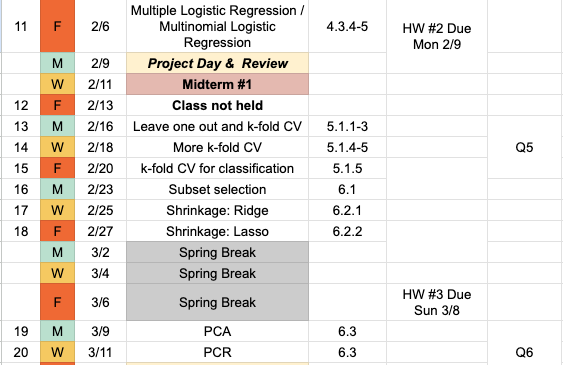
\includegraphics[alt={Screenshot of the course schedule from lectures 11 to 20.},align = c, width = \textwidth]{Schedule-S26-Lecs11_to_20}
	\centering

	\vspace{.2in}

	
	\column{.5\textwidth}
	\centering
	\textbf{Last Time:}

	\begin{itemize}
		\item  Finished Linear Regression
	\end{itemize}
	\textbf{Announcements:}
	\begin{itemize}
		\item Homework \#2 Due Sunday Feb 8
		\item Next Monday - Review day
		\begin{itemize}
			\item depends on what you ask! 
		\end{itemize}
		\item Wed 2/11 - Exam \#1 
		\begin{itemize}
			\item Bring 8.5x11 sheet of paper 
			\item \textbf{Handwritten} both sides 
			\item Anything you want on it, but must be your work 
			\item Must have your name and group number
			\item You must turn it in
		\end{itemize}
	\end{itemize}
	\end{columns}
\end{frame}
%--- Next Frame ---%
\begin{frame}[c]{Covered in this lecture }

\begin{columns}
\column{.4\textwidth}
\centering
\begin{itemize}
	\item Ch 2.2.3 
	\item Error rate (classification)
	\item Bayes Classifier
	\item $K$-NN classification
\end{itemize}
\column{.4\textwidth}
\centering

\end{columns}

\end{frame}
%--- Next Frame ---%
%=================
\section{Classification Overview}
%=================

\begin{frame}[t]{What is classification }

\begin{columns}
\column{.45\textwidth}
% \centering
Classification: When the response variable is qualitative

\InstructorList{
\item qualitative: Unordered set
\item Examples
\InstructorList{
\item Eye color $\in \{ brown, blue, green\}$
\item $email \in \{ spam, not spam\}$
}
}
\column{.45\textwidth}
% \centering
\begin{itemize}
	\item
Given feature vector $X$ and qualitative response $Y$ in the set $S$, the goal is to find a function (classifier) $C(X)$ taking $X$ as input and predicting its value for $Y$.

	\item
We are more interested in estimating the probabilities that X belongs to each category
\end{itemize}
\end{columns}

\end{frame}
%--- Next Frame ---%
\begin{frame}[c]{Some examples }

\InstructorNotes{Discuss what set $Y$ comes from in each case }

\begin{columns}
\column{.45\textwidth}
\centering
\begin{itemize}
	\item Predict whether a COVID19 vaccine will work on a patient given patient's age
	\item An online banking service wants to determine whether a transaction being performed is fraudulent on the basis of the user's IP address, past transactions, etc.
	% \item

\end{itemize}
\column{.45\textwidth}
\centering

\end{columns}

\end{frame}
%--- Next Frame ---%

%--- Next Frame ---%
\section{Ch 2.2.3: Classification}
\begin{frame}[t]{Error rate}



\begin{columns}
\column{.5\textwidth}
\centering
\begin{itemize}
	\item
Training data:

$\{ (x_1,y_1),\cdots,(x_n,y_n) \}$ with $y_i$ qualitative

\item Estimate $\hat y = \hat f (x)$
\item Indicator variable
% \vspace{.5in}

\InstructorNotes{$\mathrm{I}(y_i \neq \hat y_i)$ is 1 if not the same (misclassified) and 0 else}
% \item
\end{itemize}

\column{.4\textwidth}
Training error rate:
\begin{equation*}
\frac{1}{n} \sum_{i = 1}^n \mathrm{I}(y_i \neq \hat y_i)
\end{equation*}

Test error rate:
\begin{equation*}
	\mathrm{Ave}(\mathrm{I} (y_0 \neq \hat y_0))
\end{equation*}

\InstructorNotes{Good classifier: one that minimizes test error rate}

% \vspace{1.5in}
\end{columns}

\end{frame}
%--- Next Frame ---%


\begin{frame}[c]{Best ever classifier }
	\framesubtitle{We can't have nice things}

\begin{columns}
\column{.4\textwidth}
% \centering
\textbf{Bayes Classifier:}

Give every observation the \emph{highest probability} class given its predictor variables
\begin{equation*}
	\Pr (Y = j \mid X = x_0)
\end{equation*}
\column{.4\textwidth}
\centering
\InstructorList{
  \item It is possible to show (though the proof is outside of the scope of this
  book) that the test error rate  is minimized, on average, by a
  very simple classifier that assigns each observation to the most likely class,
  given its predictor values.
}

\end{columns}

\end{frame}
%--- Next Frame ---%

\begin{frame}[c]{An example }

\begin{columns}
\column{.5\textwidth}
\centering
\begin{itemize}
	\item Survey students for amount of programming experience, and current GPA
	\item Try to predict if they will pass CMSE 381.
	\item If we have a survey of all students that could ever exist, we can determine the probability of failure given combo of those features.
\end{itemize}
\column{.4\textwidth}
\centering
\InstructorList{
\item No single classifier will get it right 100\% since students with the same features might pass or fail
}
\end{columns}

\end{frame}
%--- Next Frame ---%

\begin{frame}[t]{Bayes decision boundary}

\begin{columns}
\column{.5\textwidth}
\centering
	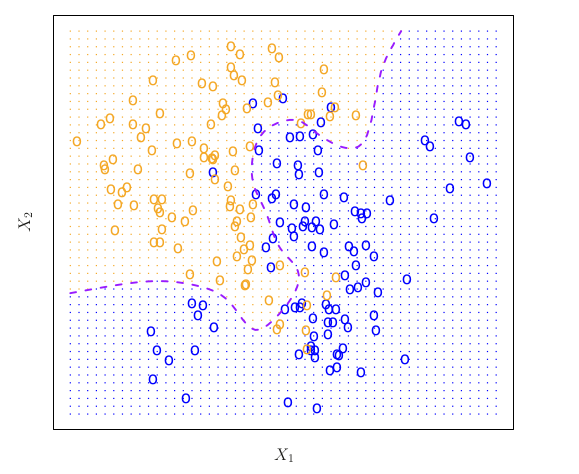
\includegraphics[alt={Data points belonging to two classes (yellow circles versus blue circles) plotted versus predictoes X1 and X2. Bayes decision boundary is also shown.},width = \textwidth]{Fig2-13.png}

\column{.4\textwidth}
\centering
\InstructorList{
\item Example where we simulated the data, so we know the conditional probability of each value of $X_1$ and $X_2$, using Bayes Theorem:
\begin{align*}
	&P(Blue|X_1,X_2) \\
	&= \dfrac{P(X_1,X_2|Blue)P(Blue)}{P(X_1,X_2)}\\
	&Posterior\\
	&= \dfrac{likelihood \cdot prior}{marginal}
\end{align*}
\item The purple line is where we switch our predictor, called the Bayes decision boundary
}
\end{columns}

\end{frame}
%--- Next Frame ---%
%--- Next Frame ---%


\begin{frame}[t]{Bayes error rate}

\begin{columns}

\column{.5\textwidth}
\centering
\begin{itemize}
	\item Error at $X = x_0$
	\InstructorNotes{The $j$ with the highest value is what's predicted by Bayes for that $x_0$, so this is probability that the Bayes classifier is wrong}
	\begin{equation*}
		1 - \max_j \Pr(Y = j \mid X = x_0)
	\end{equation*}
	\item Overall Bayes error:
	\InstructorNotes{This is expectation over all $x_0$. This is the analagous to irreduceable error}
	\begin{equation*}
		1 - E \left(\max_j \Pr(Y = j \mid X = x_0) \right)
	\end{equation*}

	\InstructorNotes{This is the irreduceable error}
\end{itemize}

\column{.4\textwidth}
\centering
	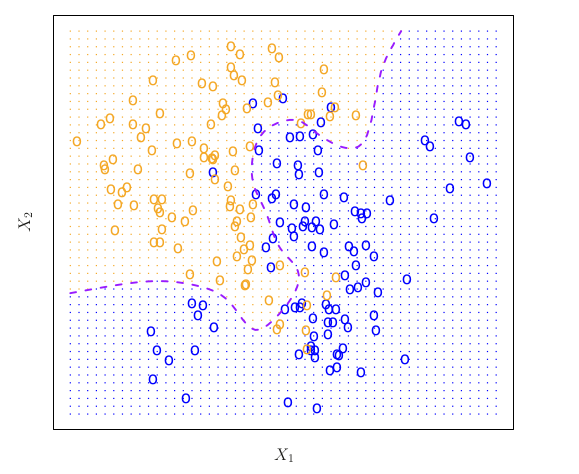
\includegraphics[alt={Data points belonging to two classes (yellow circles versus blue circles) plotted versus predictoes X1 and X2. Bayes decision boundary is also shown.},width = \textwidth]{Fig2-13.png}
\end{columns}

\end{frame}
%--- Next Frame ---%
\begin{frame}[t]{The game }
	\begin{columns}
	\column{.5\textwidth}
	\InstructorList{
	\item Challenge: typically don't know the ground truth likelihood
	\item Game: do as good a job as possible estimating the Bayes decision boundary, by guessing the posterior $P(Blue|X_1,X_2)$ and $P(Yellow|X_1,X_2)$
	\item Classify given observation with highest estimated probability
	}
	

	\column{.4\textwidth}
	\centering
	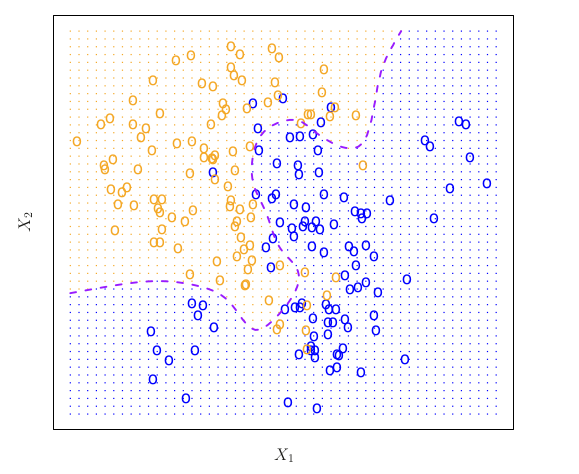
\includegraphics[alt={Data points belonging to two classes (yellow circles versus blue circles) plotted versus predictoes X1 and X2. Bayes decision boundary is also shown.},width = \textwidth]{Fig2-13.png}
	
	\end{columns}
\end{frame}
%--- Next Frame ---%

%=================
\section{$K$-Nearest Neighbors Classifier}
%=================


\begin{frame}[t]{$K$-Nearest Neighbors}


\begin{columns}
\column{.2\textwidth}
\centering
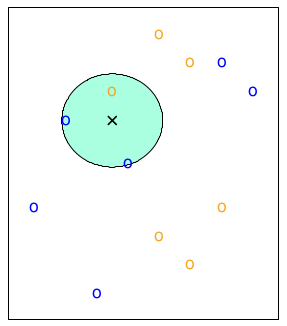
\includegraphics[alt={A plot of two classes (yellow circles and blue circles) in the plane. A test point is marked with X, and its three neares neighbors (K=3) are encolosed in a green disk.},width = \textwidth]{Fig2-14a}

$K = 3$
\column{.5\textwidth}
\centering
\begin{itemize}
	\item Fix $K$ positive integer
	\item $N(x) = $ the set of $K$ closest neighbors to $x$
	\item Estimate conditional proability
	\begin{equation*}
		\Pr(Y = j \mid X = x_0)
		= \frac{1}{K} \sum_{i \in N(x_0)} \mathrm{I}(y_i = j)
	\end{equation*}
	\item Pick $j$ with highest value
\end{itemize}
\column{.2\textwidth}
\centering
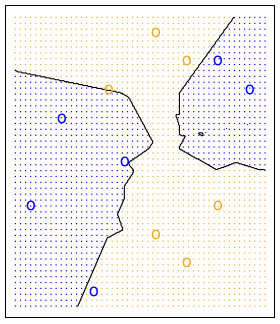
\includegraphics[alt={A plot of two classes (yellow circles and blue circles) in the plane, and the KNN decision boundary.},width = \textwidth]{Fig2-14b}

Black line: KNN decision boundary

\InstructorNotes{Note this is not Bayes like in 2 slides! stupid textbook}
\end{columns}

\end{frame}
%--- Next Frame ---%
{
  \setbeamercolor{background canvas}{bg=Apricot!25}
\begin{frame}[t]{Example}
Here label is shown by O vs X. What are the knn predictions for points $A$, $B$ and $C$ for $k=1$ or $k=3$? \InstructorNotes{Next year, maybe make an example like this with more than two levels, and/or try to decide what locations get which predictions for k=1 in prep for the next slide}
\begin{columns}
\column{.4\textwidth}
\centering

\includegraphics[alt={A 2D plot of two classes (blue circles and yellow xs). Three test points are labeled as A, B, and C.},align = c, width = \textwidth]{KNN-Example}

\column{.45\textwidth}
\centering
\begin{tabular}{c||c|c}
	               & $k=1$ & $k=3$ \\
	\textbf{Point} & Prediction & Prediction\\
	\hline 
	&& \\
	A &\InstructorNotes{O}& \InstructorNotes{O}\\
	&& \\
	B &\InstructorNotes{X}& \InstructorNotes{X}\\
	&& \\
	C &\InstructorNotes{O}& \InstructorNotes{X}\\
	&& \\
\end{tabular}
\InstructorNotes{
\includegraphics[align = c, width = .2\textwidth]{KNN-Example-Soln-K1}
\includegraphics[align = c, width = .2\textwidth]{KNN-Example-Soln-K3}
}
\end{columns}
\end{frame}
}
%--- Next Frame ---%

\begin{frame}[c]{Tradeoff}

\begin{columns}
\column{.3\textwidth}
\centering
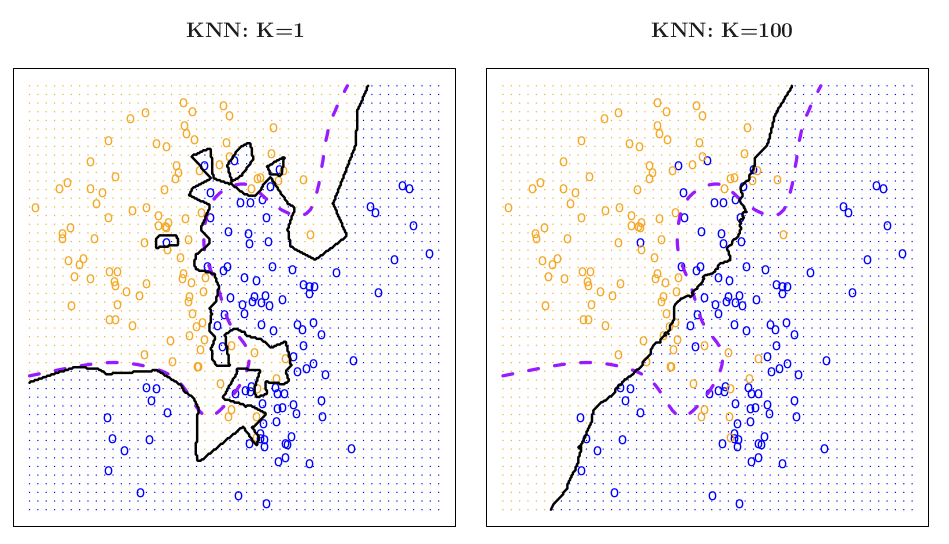
\includegraphics[alt={A plot of two classes (yellow circles and blue circles) in the plane. The KNN boundary is plotted in solid black, while Bayes decision boundary is plotted in purple.},
width = \textwidth, trim = 480 0 0 0, clip]{Fig2-16}
\column{.33\textwidth}
\centering
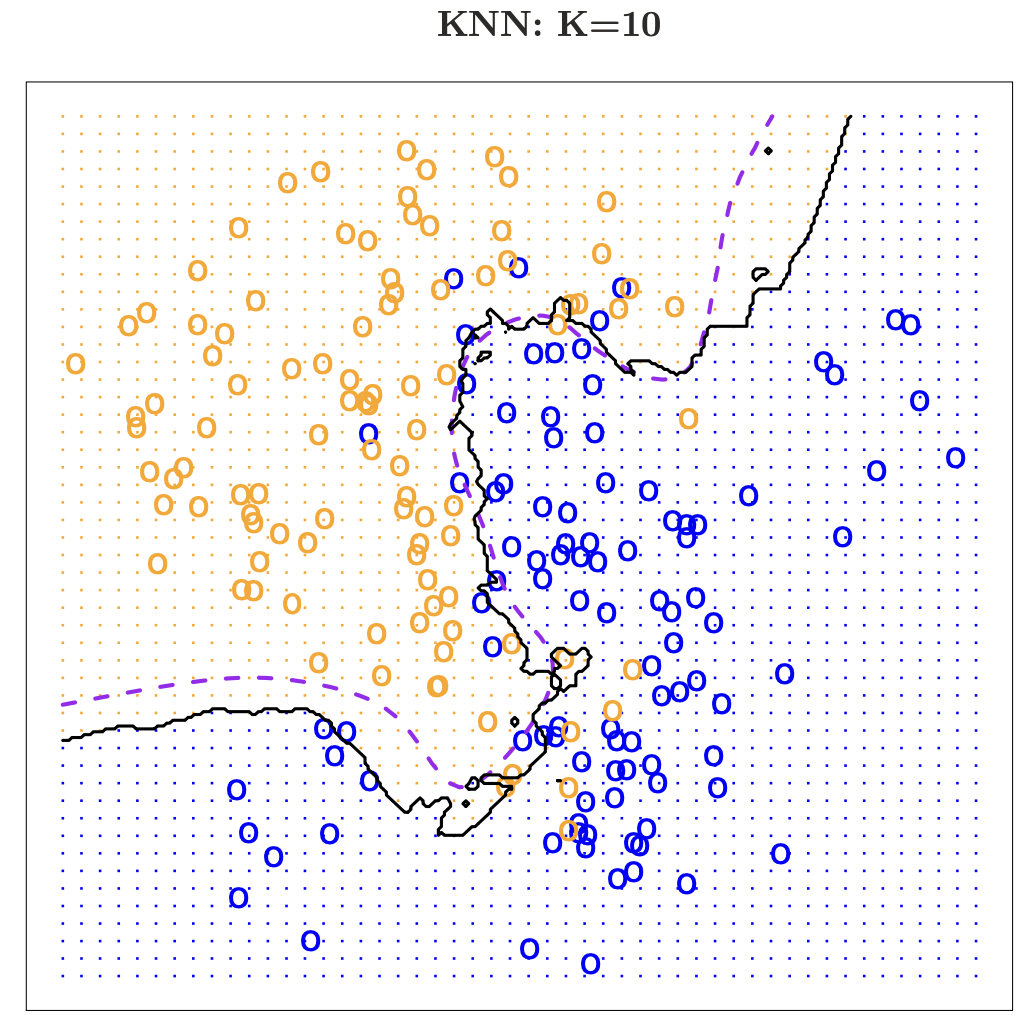
\includegraphics[alt={A plot of two classes (yellow circles and blue circles) in the plane. The KNN boundary is plotted in solid black, while Bayes decision boundary is plotted in purple.},width = \textwidth, trim = 0 0 0 0, clip]{Fig2-15}
\column{.3\textwidth}
\centering
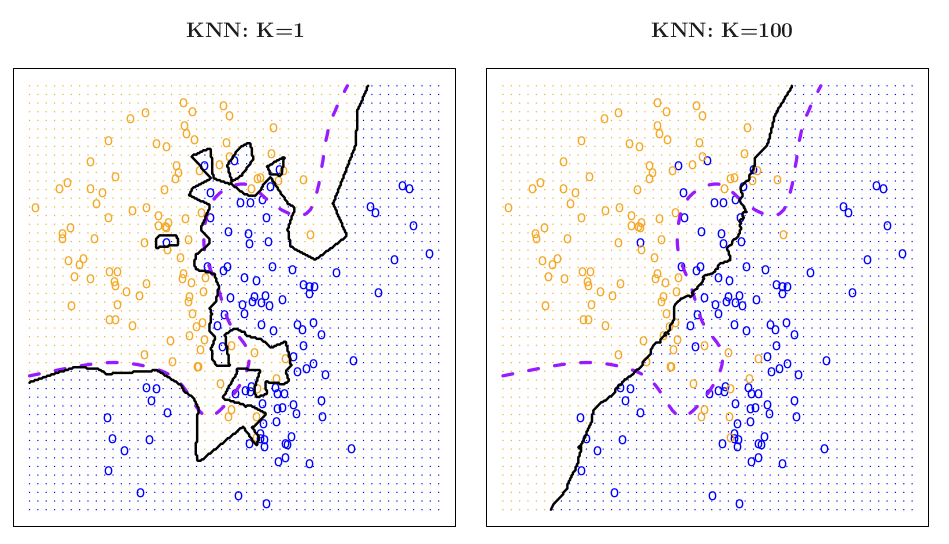
\includegraphics[alt={A plot of two classes (yellow circles and blue circles) in the plane. The KNN boundary is plotted in solid black, while Bayes decision boundary is plotted in purple.},width = \textwidth, trim = 0 0 480 0, clip]{Fig2-16}
\end{columns}
\InstructorList{
\item Purple is Bayes decision boundary. Same on both
\item $K=1$, boundary is overly flexible, finds patterns not there
\item $K=100$ not enough flexibility
}

\end{frame}
%--- Next Frame ---%
\begin{frame}[c]{More on tradeoff}

\begin{columns}
\column{.6\textwidth}
\centering
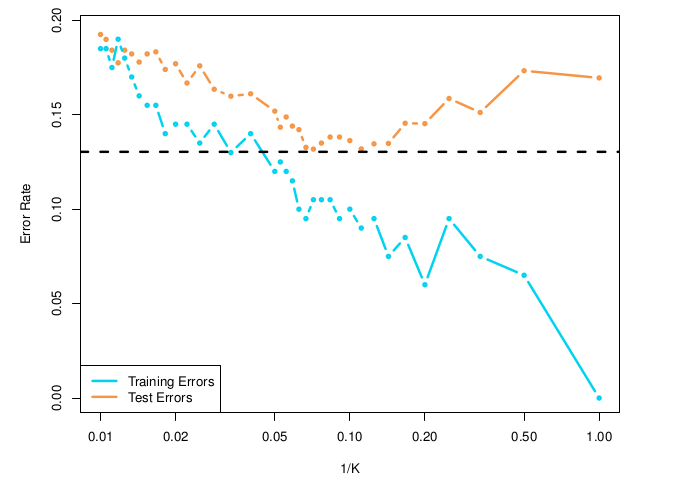
\includegraphics[alt={Training error rate (plotted in solid blue) and Test error rate (plotted in solid orange) versus 1/K.},width = \textwidth]{Fig2-17}

\column{.4\textwidth}
\centering
\InstructorList{
\item right side, $K=1$, training is 0 error but high test error
\item Test error has same U shape as bias-variance tradeoff in regression setting: decline at first, then increase again when overfitting
}
\end{columns}

\end{frame}
%--- Next Frame ---%

{
\setbeamercolor{background canvas}{bg=Apricot!25}
\begin{frame}[t]{Jupyter notebook}
\begin{columns}
\column{.45\textwidth}
\centering
\column{.45\textwidth}
\centering
\end{columns}
\end{frame}
}
%--- Next Frame ---%


% %----------------
\begin{frame}[t]{Next time}


	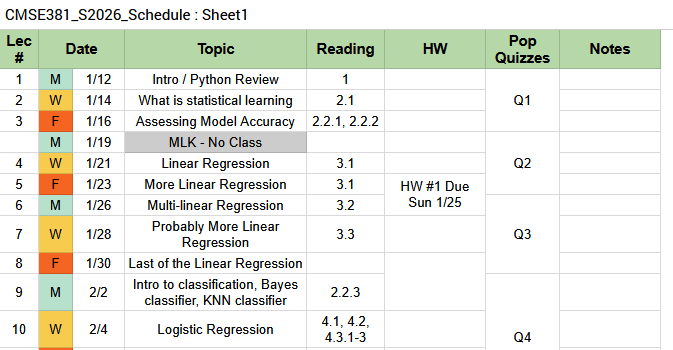
\includegraphics[alt={Screenshot of the course schedule from lectures 1 to 10.},width = .65\textwidth]{Schedule-S26-Lecs1_to_10}
\end{frame}
%--- Next Frame ---%


\end{document}
